
                                                                               \documentclass[tikz]{standalone}
\usepackage{lmodern}
\usepackage[algoruled,vlined,linesnumbered,titlenotnumbered,noend]{algorithm2e}
\usepackage{color,amsmath,bm,bbm,stmaryrd,amssymb,pifont,bbding}
\usetikzlibrary{backgrounds}
\usetikzlibrary{calc} 

\usetikzlibrary{shapes}
\usetikzlibrary{shadows}
\usetikzlibrary{decorations.pathmorphing}
\usetikzlibrary{decorations.text}
\usetikzlibrary{decorations}
\usetikzlibrary{arrows,bending}
\usetikzlibrary{shapes.arrows}
\tikzset{nobg/.style={show background rectangle,background rectangle/.style={opacity=0}}}


\input ../../styles
\input ../../globalcomm
\input ../../localcomm
\usetikzlibrary{arrows, shapes.gates.logic.US, calc}

  \tikzstyle{bddnode}=[draw,rectangle,rounded corners=2mm]
  \tikzstyle{aops}=[pos=0.9,below,yshift=0mm,xshift=-2mm]
\begin{document}



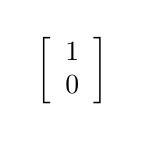
\begin{tikzpicture}
\node[] at (0,0)
     {
       $\left[
         \begin{array}{c} 1\\0\end{array}
             \right]$
       };
\end{tikzpicture}


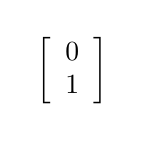
\begin{tikzpicture}
\node[] at (0,0)
     {
       $\left[
         \begin{array}{c} 0\\1\end{array}
             \right]$
       };
\end{tikzpicture}


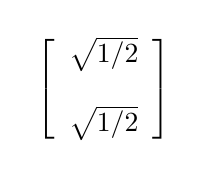
\begin{tikzpicture}
\node[] at (0,0)
     {
       $\left[
         \begin{array}{c} 
           \sqrt { 1/ 2}
           \\\\
           \sqrt { 1/2}
         \end{array}
           \right]$
       };
\end{tikzpicture}


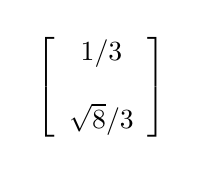
\begin{tikzpicture}
\node[] at (0,0)
     {
       $\left[
         \begin{array}{c} 
           1/3
           \\\\
           {\sqrt8}/3 
         \end{array}
           \right]$
       };
\end{tikzpicture}

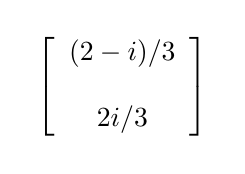
\begin{tikzpicture}
\node[] at (0,0)
     {
       $\left[
         \begin{array}{c} 
           (2-i)/3
           \\\\
           {2i}/3 
         \end{array}
           \right]$
       };
\end{tikzpicture}


\begin{tikzpicture}
\node[] at (0,0)
     {$\katof0$};
\end{tikzpicture}


\begin{tikzpicture}
\node[] at (0,0)
     {$\katof1$};
\end{tikzpicture}



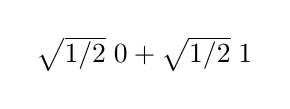
\begin{tikzpicture}
\node[] at (0,0)
     {$\sqrt{1/2}\;\katof0+\sqrt{1/2}\;\katof1$};
\end{tikzpicture}

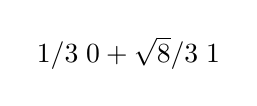
\begin{tikzpicture}
\node[] at (0,0)
     {$1/3\;\katof0+\sqrt8/3\;\katof1$};
\end{tikzpicture}

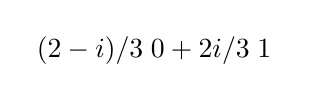
\begin{tikzpicture}
\node[] at (0,0)
     {$(2-i)/3\;\katof0+2i/3\;\katof1$};
\end{tikzpicture}


\end{document}

